\chapter{Описание постановки задачи на курсовую работу}
\label{cha:Osnovania}


\section{План работ}

\begin{enumerate}
    \item Ознакомится с литературой.
    \item Сформулировать цель и задачи работы.
    \item Сделать переход от вида с камеры на вид сверху (Projective Geometry).
    \item Решить TSP-задачу для обхода статично располагающихся на поле игроков.
    \item Разработать симуляцию для отладки и тестирования алгоритма управления длиннофокусной камеры.
    \begin{enumerate}
        \item Обработать заранее размеченные данные для построения тепловой карты перемещения игроков.
        \item На основе тепловых карт реализовать модель перемещения игроков по полю, максимально соответствующую их перемещению в реальной игре.
        \item Разработать симуляции камерной проекции на поле (3D).
        \item Разработать API для управления камерой в симуляции.
        \item Объединить симуляцию поведения объектов с симуляцией камеры.
    \end{enumerate}
    \item Разработать метрику, справедливо оценивающую работу алгоритма.
    \item Разработать алгоритм управления камерой, имеющий лучшие показатели точности.
    \begin{enumerate}
        \item Реализовать обход поля по точкам, которые являются наиболее посещаемыми каждым из игроков без прогноза движения игроков (по каждому игроку найти самую частую точку).
        \item Представить движение камеры как суперпозицию движения камеры между зонами и в системе отсчета, связанной с очередной зоной.
        \item Реализовать обход игроков с учетом прогноза движения игроков.
    \end{enumerate}
    \item Реализовать модель PTZ камеры с учетом ограничений накладываемых на ее скорость и ускорение. В простейшем случае  колебаниями пренебрегаем.
    \item Подытожить результаты.
\end{enumerate}


предположения:

1) данные на вход достаточно хорошо размечены и отображают справедливые локации объектов, id не перемешиваются

2) одна камера имеет обзор на все поле, вторая - длиннофокусная

3) если лицо повернуто на +- 45 градусов , к камере, считается, что возможно фотографирование

4) рост игроков - 170 с возможностью задания индивидуальных значений 

5) вместо игроков можно показывать палочки с овалами сверху (имитация лица) \href{https://www.google.com/search?q=siluette+socer&oq=siluette+socer&aqs=chrome..69i57j0i13i512l9.8195j0j15&sourceid=chrome&ie=UTF-8#vhid=VlKJM8sBEGAFAM&vssid=l}{а че не так} - потому что курсовая работа не об этом, это короткий ответ, если подробнее - то это добавляет много сложности и нужно искать специфические библиотеки, которые могут не поддерживаться остальным проектом.

6) если лицо попало в 150 пикселов при условии пункта 3 и его не загораживают другие игроки, игрок отснят

Сделать:

1) вид с PTZ  камеры  

2) сделать блок схему пайплайна  в латех

3) попробовать брать подмножество игроков и оптимизировать на них - это зачем??? - это совет от вашего коллеги, брать всех игроков бывает вычислительно-сложно, можно брать подмножество

4) зум на игроков, так, чтобы 150 пикселов приходилось на лицо

5) замерить среднюю скорость greedy алгоритма- тоже не понял - замерить скорость нашего жадного KNN алгоритма, который уже готов (10.05 дата) на нескольких симуляциях, чтобы оценить среднее выполнение на фиксированном наборе игроков.

6) доделать симуляцию игроков

7) написать результаты

% 7. Создание двумерной проекции 


\section{Постановка задачи}

Разработать механизм управления длиннофокусной камерой для эффективного обнаружения и отслеживания игроков в поле зрения. Предлагается циклический процесс, в рамках которого камера автоматически переключается между игроками, корректируя угол обзора и дистанцию съемки. В начале каждой итерации камера сфокусирована на новом игроке, дистанция между ним и камерой оптимизируется до тех пор, пока силуэт или лицо игрока не займет заданное количество экранного пространства - n\% (c учетом допуска). После этого камера фиксируется на игроке на определенное количество кадров k, после чего переходит к следующему игроку для следующей итерации процесса.

При использовании термина `эффективно`  в данном контексте подразумевается, что алгоритм должен оперировать наилучшим образом на различных наборах данных, таких как видеозаписи футбольных матчей с метками игроков и их позициями на каждом кадре. Алгоритм, протестированный на под-выборке взятой из генеральной совокупности футбольных матчей, должен выполнять обход со съемкой за кратчайшее время.

\subsection{Преобразование Координат}
The first task is to create a coordinate mapping between the given video recording of a football match and the 2-D view from above the field. 
% Task is to convert coordinates $(x,y)$ resembling pixels on a video, that were obtained from a video-camera to $(\hat{x}, \hat{y})$ coordinates of a football field from a top view perspective.

More formally, given vector space $C$, representing camera coordinates, and vector space $P$, which represents 2-D plane coordinates, find a map between the two vector spaces $f:C \rightarrow P$ such that: 
$$
\forall c \in C \quad \exists! p \in P 
$$

\textcolor{blue} {A projectivity from a projective plane to a projective plane is called a plane-to-plane projectivity, although it is often referred to by simply using the more general term of projectivity. It acts on, and generates, a homogeneous 3-vector and is therefore a 3-by-3 matrix.
To see how such a projectivity arises, consider two images taken from different viewpoints of a plane in a scene, Figure 1. The mapping of points on to the corresponding points in image 1 is described by a projectivity . Similarly, the mapping of points on to the corresponding points in image 2 is described by a projectivity . An important property of projectivities is that they form a group. It follows that there is a projectivity which describes the mapping of the image of in image 1 to the image of in image 2, where} 
$$ R = ST^{-1}$$

Given particular coordinates $X,\;Y$ a plane-to-plane projective transformation can be done as following:

$$
\begin{bmatrix}
\tau_{i}X' \\
\tau_{i}Y' \\
\tau_{i}
\end{bmatrix} = 
\underbrace{ \begin{bmatrix}
a_{1} & a_{2} & b_{1} \\
a_{3} & a_{4} & b_{2} \\
c_{1} & c_{2} & 1
\end{bmatrix} }_{ M } \begin{bmatrix}
X \\
Y \\
1
\end{bmatrix}
$$

Where $a_i$ are elements of a scaling/rotation matrix, $\begin{bmatrix}
    b_2 & b_1
\end{bmatrix}^T$ is a translation vector and $\begin{bmatrix}
    c_1 & c_2
\end{bmatrix}$ is a projection vector.

To find true new coordinates $X', Y'$ resulting vector has to be divided by $\tau_i$ that is the scaling factor. 

\subsubsection{Code implementation}

Given source image field corner coordinates in a list corner\_src\_points, a projective transformation matrix can be calculated. Function cv2.getPerspectiveTransform takes 2 arguments: source (4 coordinates (x,y), resembling corners of the input quadrilateral) and destination (4 coordinates (x,y), resembling corners of the output quadrilateral). On output the projective transformation matrix $M \in \mathbb{R}^{3 \times 3}$ described above is obtained.

\lstinputlisting[language=Python]{listings/projective_matrix.py}
\lstinputlisting[language=Python]{listings/coordinates_trans.py}
% add a link to library
Now by using this function and warpPerspective function from \textcolor{purple}{opencv} library, transformation can be done:
\begin{lstlisting}
corrected_image = cv2.warpPerspective(image, M, (width, height), borderValue=(255,255,255))
transform_coordinates(file_name="unscaled_track_df_new_coords.csv")
\end{lstlisting}


\section{Структура используемых данных}

Дано футбольное поле на котором находятся игроки и мяч, заданные координатами $\vec X$, как функциями времени $t$,  в системе отсчета, связанной с полем. Таким образом у нас есть входной массив $X^{nm}_i$, где 

$n$ - номер игрока;

$m$ - описывает одну из координат положения игрока;

$i$ - описывает момент времени. 

Необходимо построить функцию управления осью камеры высокого разрешения (зарезервируем $k$ для номера камеры) с заданными характеристиками:

$F=(F_{min},F_{max})$ - диапазон изменения фокусного расстояния;

$U=(u_1,u_2)$ - размер матрицы камеры в пикселах;

$p$ - размер пиксела матрицы в метрах (real world size of an image sensor's pixel);

$\Omega=(\omega_1, \omega_2)$ - максимальная угловая скорость по углу места и азимуту;

$\frac{dF}{dt}_{max}$ - максимальная скорость изменения фокусного расстояния во времени.  

Координаты камеры в системе отсчета связанной с левым дальним углом поля 

$$W=\{w_1,w_2,w_3\}$$

%Перенести в список терминов и определений

\subsection{Фокусное расстояние (Focal Length)}
Focal length is a distance between "nodal point" (that is where light converges in a lens) and a camera sensor\cite{FocalLength}. Cameras have a base focal length (max), but some cameras provide with a possibility to vary focal length by increasing/decreasing length of an objective (объектив). Thus a range of focal length ($F=(F_{min},F_{max})$) is of interest, as applications imply usages with long focus lenses.

 \begin{figure}[!htbp]
     \centering
     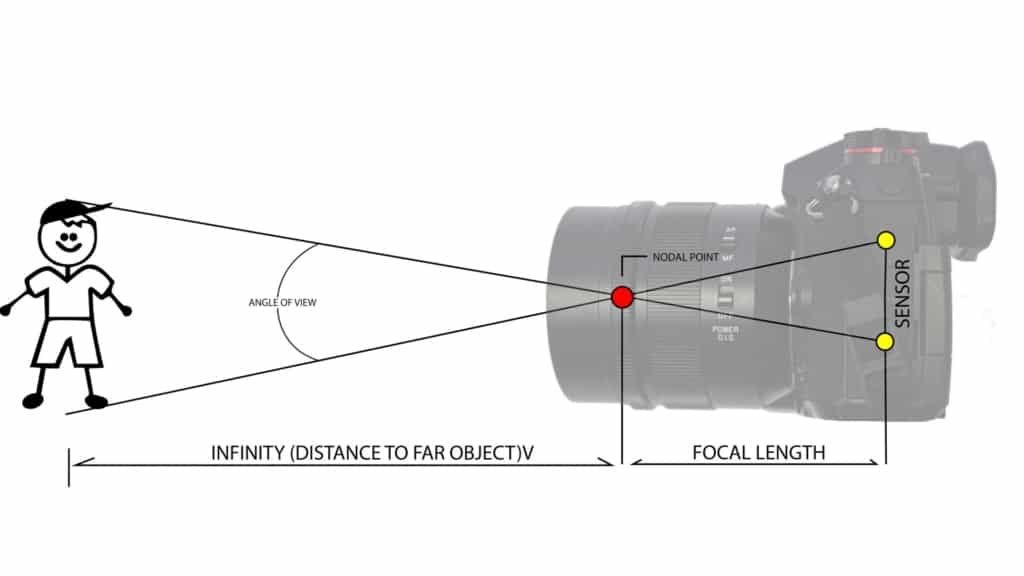
\includegraphics[width=0.8\linewidth]{figures/focal.jpg}
     \caption{Focal Length}
     \label{fig:enter-label}
 \end{figure}

\subsection{Матрица камеры (Image sensor)}
 An image sensor refers to the electronic component in a digital camera that captures and converts light into digital signals, ultimately creating a digital image. The image sensor plays a crucial role in digital photography by replacing the traditional film used in film cameras. $U=(u_1,u_2)$ - sensor size of a camera in pixels represents number of pixels along $x$ and $y$ axes respectively, total image might have upmost $u_1*u_2$ pixels, given that photo is RGB, it can be calculated, that on an 3-dimensional tensor with shape $(u_1, u_2, 3)$ the whole image can be stored, and on 4-dimensional tensor with shape $(u_1, u_2, 3, \textbf{frames})$ a whole video may be stored frome such camera without audio-stream, where frames - is the amount of frames taken from that camera consequently.



\subsection{Угловая Скорость (Angular Velocity)}
An angular velocity is the speed of rotation for an object that can be stated as ${\displaystyle \omega ={\frac {d\varphi }{dt}}}$.

\subsection{Угол Места; Элевация (Elevation)}
Vertical angle of an observed object over true horizon. Elevation combined with azimuth are used for obtaining the direction to an object. \href{https://ru.wikipedia.org/wiki/%D0%A3%D0%B3%D0%BE%D0%BB_%D0%BC%D0%B5%D1%81%D1%82%D0%B0}{Elevation}

\subsection{Азимут (Azimuth)}
Horizontal angle evaluated from predefined direction (for example north) and direction of an observed object.

\section{Простейшая задача управления камерой высокого разрешения}

Необходимо предложить алгоритм обхода всех игроков на поле начиная с центра поля.

В результате мы должны получить:

$\vec \psi(t)$ - вектор, описывающий угол места и азимут визирования камеры, как функцию времени. 

При этом мы должны обеспечить получение изображения игрока в поле зрения камеры в течение времени $\Delta T$ соответствующего $R$ кадрам. 

Движение игроков считаем априорно неизвестным. 

1) Первый шаг - обход неподвижных игроков

2) Второй шаг - обход движущихся игроков 

\subsection{Обход неподвижных игроков}

Дан взвешенный граф $G = (V, E)$, в нашем случае полный, поскольку от любой вершины может быть рационально перейти к другой, в общем случае, где

$V$ - количество распознанных на кадре объектов, на данном этапе футболистов, $V = {1, 2, 3, ..., k}$

$E$ - ребра данного графа; 

$d_{ij}(i, j \in V, i \neq j)$ - расстояние между двумя вершинами $i, j$, причем $d_{ij} > 0$,  $d_{ij} \neq \infty$ и $d_{ij} = d_{ji}$.

Требуется найти такой гамильтонов цикл (замкнутый путь), что 
\begin{align}
    minD  = \sum_{i,j \in V} d_{ij} * x_{ij},
\end{align}
где 
\begin{equation}
    x_{ij} = 
    \begin{cases}
        1 & e_{ij} \in \text{оптимальный путь}\\
        0 & e_{ij} \notin \text{оптимальный путь}
    \end{cases}
\end{equation}
То есть $x_{ij}$ - это логическая переменная, обращающаяся в 1, если ребро $e_{ij}$ удовлетворяет условию принадлежности оптимальному пути, и 0 иначе. Начало и конец обхода, в общем случае, происходят в центре футбольного поля. Результатом работы алгоритма должен быть путь, содержащий в себе все вершины графа и удовлетворяющий условиям, заданным выше.

\section{Приближения и ограничения}
 
Перемещение угла камеры вверх/вниз влево/право и фокусировка не зависят друг от друга и могут выполняться параллельно. (От этого зависит метрика оптимизируемая)

 
Мы планируем иметь количество объектов другое и сильно большее, чем количество футболистов. (От этого зависит выбор алгоритма - так как задача NP трудная то для малого количества её можно решать в лоб - гипотеза на 22 в лоб оптимальнее)

Камера должна возвращаться в исходную точку (по умолчанию - в центр). 

 
Считать что скорость бега футболиста пренебрежимо мала относительно скорости камеры нельзя.  
